\section{Robot Operating System 2 (ROS 2)}
A ROS (Robot Operating System) egy nyílt forráskódú middleware, robotikai keretrendszer. Nem teljes értékű operációs rendszer, ahogy a nevéből gondolni lehetne, hanem a robotfejlesztéshez szükséges szoftverkeretrendszerek halmaza. A munkám során ROS 2 Humble verzióját használtam, ezért a fejezetben a ROS 2 funkcióit és koncepciót ennek a verziónak megfelelően mutatom be. \cite{ros2} \cite{ros2_article}

A ROS 2 egy továbbfejlesztett változata a ROS-nak, amelyet a modern robotika követelményeinek figyelembevételével terveztek újra. a Főbb különbségei közé tartozik a valós idejű működés támogatása, a jobb biztonsági és több szálú működés képességei, valamint a DDS (Data Distribution Service) használata a belső üzenetküldéshez, kommunikációhoz. Míg a ROS 1 a Master-Slave architektúrát használja, addig a ROS 2 a Data Distribution Service (DDS) rendszert alkalmazza, amely nagyobb megbízhatóságot, alacsonyabb késleltetést és jobb skálázhatóságot kínál. A DDS elosztott jellege lehetővé teszi a kommunikációs hibák minimalizálását, valamint támogatja a valós idejű rendszereket. Továbbá, míg a ROS 1-ben két külön könyvtár (roscpp és rospy) létezett, addig a ROS 2 központi, C nyelven íródott rcl könyvtárat használ, amely több programozási nyelvet is támogat, például Python, C++, Java és C\#. A ROS 2 ezenkívül jelentős fejlődést hozott az adatformátum kezelésében is, amely több rugalmasságot kínál a szerializálás terén a belső folyamatok kommunikációjában. A ROS 2 új funkciói közé tartozik a QoS (Minőségbiztosítás) támogatása. Ez magában foglalja az üzenetek megbízhatóságára, határidejére és prioritására vonatkozó beállításokat, amelyek biztosíthatják, hogy a kritikus üzenetek időben kézbesítésre kerüljenek. A többszálú végrehajtás lehetősége node-ok és azok belső folyamatainek párhuzamos futását teszi lehetővé. így jobban ki tudja használni a modern többmagos processzorokat, mint a ROS 1. Mindezek hozzájárulnak a valós idejű feldolgozás javításához, így sokkal jobban alkalmas a komplex, ipari robotikai alkalmazások számára. \cite{ros2} \cite{ros2_article}

Nem célom kitérni és bemutatni teljes végletében a ROS 2 alapelveit és működését, továbbiakban a diplomamunka szempontjából lényeges funckiók, koncepciók kerülnek csak kiemelésre és tárgyalásra, a többi információ a hivatalos dokumentációban megtalálható.

\subsection{Modularitás és node-ok}
ROS 2 olyan szolgáltatásokat, eszközöket nyújt, amelyek lehetővé teszik különböző számítógépekből álló rendszer hatékony együttes működtetését. Ezek közé tartozik az absztrakt hardver kezelés, rengeteg gyártó nyújt a termékükhöz (pl. szenzorokhoz, aktuátorokhoz, vagy akár teljes robotkarokhoz) ROS 2-es csomagokat és támogatást fizikai eszközhöz, gyakran szimulációs környezethez. Nyílt forráskodú, mely hozzájárul a fejlesztők közzötti együttműködéshez, a fejlesztési idő csökkentéséhez, a szoftverek újrafelhasználásához, a szabványosításhoz és a széles körű támogatáshoz. A ROS 2 alapvető építőelemei a node-ok, amelyek az alkalmazások különálló, moduláris komponensei. Minden node egy adott vagy akár több feladatot lát el, például szenzoradatok feldolgozását, mozgástervezést vagy robotvezérlést, és önállóan, más node-októl függetlenül működik. A node-ok egymással üzenetküldés útján kommunikálnak, amely lehetővé teszi az adatok hatékony megosztását, akár különböző számítógépek között is. Több kommunikációs metódus megvólsítható node-ok között, de a lényeg, hogy szabványosított működésüknek köszönhetően már elkészített, mások által lefejlesztett csomagok egyszrűen és viszonylag költségmentesen bővíthetőek saját fejlesztésű node-okkal. A ROS 2 megosztott architektúrája miatt a node-ok nem igényelnek központi vezérlést, ami növeli a rendszer robusztusságát és skálázhatóságát. Ezzel a koncepcióval a node-ok egyszerűen cserélhetők vagy újrahasznosíthatók, megkönnyítve a komplex robotikai rendszerek fejlesztését és bővítését. Egy node leprogramozásakoz a megfelelő nyelvspecifikus könyvtár node osztály implementációjából származtatjuk az osztályt, amely az objektum orientált programozás elveihez kötve örökli az interfészek, paraméterek, időzítők létrehozását. \cite{ros2}

\subsection{ROS 2 client library: rclpy}
Több kliens programkönyvtárat (client library-t) kínál a ROS 2, amelyek lehetővé teszik a fejlesztők számára a ROS 2 rendszerrel való kommunikációt. Több nyelven biztosít klienskönyvtárat, például a kettő legelterjedtebb: C++, Python. Fejlesztői döntés alapján választható, hogy melyi megfelelőbb egy felhasználói esetre. Ha egy gyors és hatékony megoldásra van szükség, akkor egyértelműen a C++-os klienskönyvtár a megfelelő választás, ha viszont a fejlesztési idő csökkentése és a könnyű használhatóság a cél, akár egy adatvizualizációs vagy fájlkezelési problémára, akkor a Python klienskönyvtár a megfelelő választás.

\begin{figure}[!ht]
    \centering
    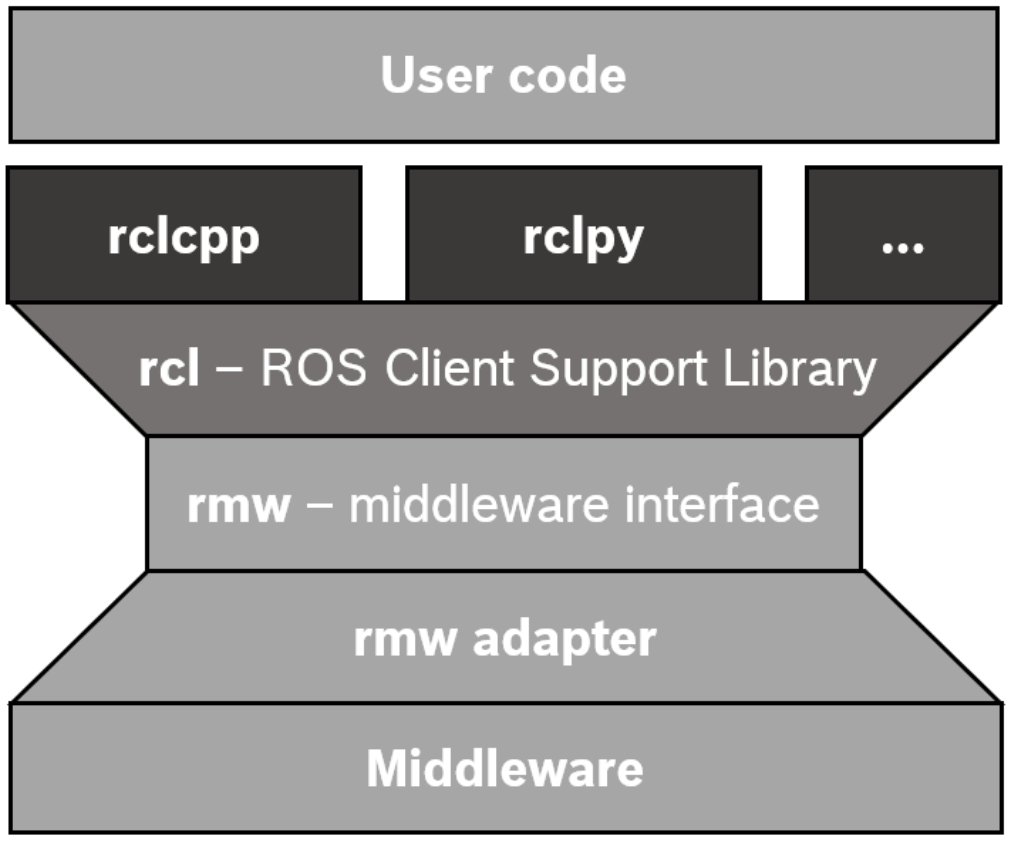
\includegraphics[width=75mm, keepaspectratio]{figures/031_rclpy.png}
    \caption{Client library arhitektúra \cite{ros2}}
    \label{fig:031_rclpy}
\end{figure}

A Python nyelvhez a rclpy csomagot használtam, amely a ROS 2 Python klienskönyvtára. Az rcl C-ben írodott API alapjaira épül és natív Python-os adatstruktúrákat használ. Külön Python kódot generál mindegy egyes ROS 2 üzenet típushoz és az ezekből létrehozott objektumokat fordítja C nyelvre, ha tovább kell küldenie az rcl rétegnek, adattovábbítás céljából. A rclpy csomag, mint client library, lehetővé teszi a Python programok számára, hogy kommunikáljanak a ROS 2 rendszerrel (\refstruc{fig:031_rclpy}), például node-okat hozzanak létre, üzeneteket publikáljanak és feliratkozzanak, szolgáltatásokat hozzanak létre, paramétereket kezeljenek, módosítsanak, szimulációs időhöz férjenek hozzá. Biztosítja a logging lehetőségét és szálkezelési modellt. \cite{ros2}

\subsection{Launch fájlok}
A ROS 2-es launch rendszer célja, hogy a felhasználó számára átláthatóvá tegye és összefoglalja node-ok indítását, paraméterezését és konfigurálását. Ezen kívül a rendszer figyelemmel kíséri (összeszedet logolást biztosít) és esetlegesen reagál a változásokra. A nagyobb rendszerek konfigurációja összetett lehet, ezért a launch rendszer egyik fő előnye a moduláris konfigurációk és az al újrafelhasználhatóság támogatása. Úgynevezett launch fileok írhatóak XML vagy Python nyelven. Lehetőséget biztosítanak az indítási paraméterek meghatározására (TODO: késsőbiekben részletesen), namespace-ek létrehozására (node-ok és paraméterek elkülönítése céljából), interfészek csoportosítására illetve remapping-ek készítésére (topic-ok és service-ek nevének megváltoztatására). Launch argumentumok azaz launch fájloknak megadható paraméterek (nem node paraméterek) definiálhatóak, amikből akár feltételes node indítást lehet leprogramozni, vagy különböző konfigurációk betöltése vezérelhető vagy fájlok elérési útvonala változtatható meg. Launch fájlok segítségével tehát egyszerre indítható és állítható le több node. Futás közben monitorozható és futás után log fájl megtekintésével debugolható. Rengeteg előnyt biztosítanak tehát a launch fájlok. Ebben az összefoglalóban szintén a részletekre nem, csak a munka szmepontjából lényeges tulajdonságokra tértem ki. \cite{ros2} \cite{ros2_design}

\subsection{Interfészek}
A ROS 2 alkalmazások, node-ok jellemzően háromféle interfész típuson keresztül kommunikálnak: messages, services, és actions. Ezek leírására a ROS 2 egy egyszerűsített interfészleíró nyelvet (IDL) használ, amely megkönnyíti az interfész típusának forráskód-generálását több programozási nyelvre. Az IDL lehetővé teszi, hogy az interfészek adattípusai egyszer legyenek megírva szabványosított formátumban és az ezekből generált különböző nyelvű forráskód autómatikusan történjen. Minden node-nak lehet több különböző interfésze és típusunkont és bármennyi.

A publisher-subscriber kommunikációs modell a .msg típust használja. A publisher adatok továbbítására szolgál egy topic-ra, amelyet a subscriber olvas. Egy topic-ra több publisher és több subscriber is csatlakozhat, ebben az esetben mindegy egyes subscriber megkapja az üzenetet. A service-k a .srv típust használják, amely egy kérést (request) és egy választ (response) tartalmaz. A kliens küld egy kérést a szolgáltatásnak, amely válaszol a kérésre. Az action-ök a .action típust használják, amely egy kérést (goal), egy visszajelzést (feedback) és egy választ (result) tartalmaz. Az action-ök a service-ekhez hasonlóan működnek (szintén kliens-szerver modell), de megszakíthatóak és visszajelzést adnak a kliensnek a folyamat állapotáról. \cite{ros2} \cite{ros2_design}

\subsection{Paraméterek}
A paraméterek a ROS 2-ben eredendően node-okhoz kapcsolódnak. Egy node létrehozásakor definiálhatunk paramétereket, melyekkel a node futásához szükséges adatokat tárolhatunk. Ennek az implementációnak előnye, hogy modularitás és skálázhatóság elvét segíti, azaz különböző felhasználó igényeknek könnyen átszabhatóvá teszi a node-okat. Például egy szabályzó frekvenciája definiálható ilyen paraméterként, s ezáltal állíthatóvá válik különböző futás körülmények között. A paraméterek a ROS 2 node-okhoz kapcsolódnak, és azok konfigurálására szolgálnak az indításkor vagy futás közben, anélkül hogy a kódot módosítani kellene. Egy paraméter élettartama szorosan kapcsolódik a node-éhez, bár a node implementálhat olyan mechanizmusokat, amelyek az értékeket újra betöltik egy újraindítás után. Minden paraméter egy kulcsból, egy értékből és egy típusból áll, az érték különböző típusokat vehet fel. Részletesen a hivatalos dokumentációban elérhetőek a különböző típusok, amit lényeges megemlíteni, hogy a paraméterhez tartozó definit típus meggátolja, hogy futási időben a meghibásodás lehetőségét. A paraméterek nevét, típusát szükséges a node implementációjában megszabni. Az értéke opcionálisan megadható, illetve lehetőség van alapértelmezett érték megadására is. A paramétereket a node-ok indításakor is megadhatóak parancssoron, vagy node-ok launch fájlból indításakor kódból, vagy .yaml fájlból is. A paraméterek felülírhatók, tehát előre definiált alapértelmezett értéküknél egyel magasabb fokon van a launch fájl és a node "ros2 run ..." parancsal indításakor megadott érték. Ez mellett a launch fájlokban beimportált .yaml configurációs fájlokkal is felülírhatók. A .yaml fájlok nagy előnye, hogy sok paraméter esetén átláthatóbbá teszi a konfigurációt, könnyen módosítható és újrahasználható. Ugyanis egy konfigurációs fájl több node paraméterét is tárolhatja.

A paraméterek hatalmas előnye, hogy lehetőséget biztosítanak futás közbeni módosításra.  A node paramétereit futás közben API-n keresztül, vagy külső folyamatokból paraméter service-ekkel lehet módosítani. A paraméterek változását "set parameter callback" vagy "on parameter callback" függvények segítségével előre definiálni kell. Ha egyszerű értékadás történik akkor is. Ennek az az előnye, hogy olyan paraméter megváltoztatása esetén, ha olyan változik amely kihatással van a működésre (pl. frekvencia, időzítők periódusideje vagy szabályzó paraméterek) leprogramozható mi történjen a hatására. Interakcióba a paraméterekkel különféle módokon juthatunk. Egyik módja parancsoros eszköz használata a "ros2 param set/get/..." szolgáltatás, mellyel változtatni illetve értéket lekérni is tudunk. Ha autómatizálni szeretnénk, amely a diplomamunka egy fő motívuma, egy másik futó node-ból service hívással is megtehető. Minden node-hoz tartoznek service-ek amik lehetővé teszik a futás közbeni érték cserét. \cite{ros2} \cite{ros2_design}

\subsection{Executors}
TODO: kép
Az executor-ok menedzselik ROS 2-es folyamatok végrehajtását. Az executor egy olyan entitás, amely felelős a node-ok futtatásáért és események (időzítő vagy üzenet érkezés) hatására kiváltott callback-ek végrehajtásáért. Az executor-ok lehetővé teszik a node-ok párhuzamos futását. Az executorok az alap operációs rendszeren keresztül a processzor szálait használják a folyamatok futtatására. Az executor felelős a megfelelő függvények meghívásáért üzenetek vagy események feldolgozása céljából. Ellentétben a ROS 1-el, ahol a beérkező üzeneteket a klienskönyvtár szintjén tárolták sorban, a ROS 2-ben az üzenetek a köztes rétegben (rcl) maradnak, amíg a függvények feldolgozzák őket. Ez a tervezési megközelítés összhangban van a szolgáltatás minőséget biztosító (QoS) szabályokkal, biztosítva az erőforrások hatékonyabb kezelését. Az executor-ok "wait set" mechanizmust használnak a rendelkezésre álló üzenetek figyelésére és az időzítők lejártának észlelésére, így optimalizálva a visszahívások kezelését. A ROS 2 háromféle executort kínál, amelyek eltérő felhasználási esetekre vannak szabva. \cite{ros2} \cite{ros2_design}

\begin{itemize}
    \item \emph{Egyszálas executor (Single-Threaded Executor)} a legegyszerűbb executor, amely egyetlen szálat használ a függvényhívások sorozatos feldolgozására. Olyan node-okhoz ideális, ahol a párhuzamos futás nem szükséges vagy nem kívánatos. \cite{ros2}

    \item \emph{Többszálas executor (Multi-Threaded Executor)} a párhuzamosságot szem előtt tartva több szálat használ a visszahívások egyidejű feldolgozására. A szálak száma konfigurálható, lehetővé téve a teljesítmény jelentős növelését olyan rendszerekben, ahol nagy a függvényhívások száma terheli a rendszert vagy az alacsony késleltetés kritikus szempont. A párhuzamos feldolgozást a callback csoportok logikai szabályai határozzák meg. A callback csoportok abból a szempontból lényegesek, hogy ezek segítségével tudja értelmezni a folyamatok prioritását. Kétféle csoport létezik: a "Mutually exclusive", mely elemei nem futhatnak párhuzamosan és a "Reentrant", mely elemei párhuzamosan futtathatóak. Külöböző callback cosportokhoz tartozó folyamatok lefuthatnak párhuzamosan. Ennek nagy szerepe az adatok feldolgozásánál van, segítségükkel megakadályozhatók a versenyhelyzetek és a deadlock-ok. \cite{ros2}

    \item \emph{Statikus egyszálas executor (Static Single-Threaded Executor)} optimalizálja azokat az eseteket, ahol a node-ok szerkezete (pl. subcriber-ek, időzítők) nem változik a futásidő során. Csak egyszer vizsgálja meg a node felépítését az inicializáláskor, szemben a másik két executor-ral, amelyek rendszeresen újravizsgálják azt. Ezért a statikus egyszálas executor-okat csak olyan node-ok esetében ajánlott használni, amelyek minden szükséges komponenst az inicializálás során hoznak létre. \cite{ros2}
\end{itemize}

\subsection{Composition}
A composition egy olyan koncepció amely megbontja a modularitását a ROS 2-es rendszernek. Teszi ezt azért, hogy gyorsabb feldolgozást nyerjen. A megszokott külön node-okban külön folyamatok helyett a node-okat lehetőség van átalakítani és "component"-ként regisztrálni, majd többet egy "container"-be betölteni. Így külön "process"-ek helyett egyben futnak. Ezt a koncepciót azért szükséges kiemelni, mert a NAV2 használja. A composion-nel megvalósíthat az "intra-process communication" (IPC), aminek lényege, hogy ugyanazokat az adatokat használó node-ok nem üzenetekkel kommunikálnak, hanem gyakorlatilag memóriacímekkel. Tehát egy container-ben indított két node ha ugyanahhoz az adathoz akar hozzáférni, a szoksásos interface-eken keresztül megteheti viszont csak virtuálisan lesz az üzenetként elküldve. Ez helyett például egy kép feldolgozó "pipeline" működésénél az adott kép memóriába töltése után a két node ugyanúgy éri el, közöttük a a kommunikáció közvetlen memóriaozáféréssel valósul meg, így gyorsítva a feldolgozást és csökkentve az erőforrás igényt. Mivel process-ek közötti kommunikáció sokkal lassabb mint az egy process-en belüli. Az IPC segítségével a különböző folyamatok közötti kommunikáció során csökkenthető az adatmásolások száma. A memóriában elhelyezett adatokat közvetlenül is megoszthatja a rendszer a folyamatok között, minimalizálva a teljesítményveszteséget. Az IPC a zero-copy technikát használhatja, amely lehetővé teszi, hogy az adatokat közvetlenül a memóriában osztják meg a résztvevő folyamatok között, további másolási műveletek nélkül. Ez különösen hasznos, ha nagy méretű üzeneteket (például szenzoradatokat vagy képeket) kell továbbítani. Mintilyen nagy méretű szenzoradatokkal dolgozo csomag a NAV2 és különböző funkciói jelentősen profitálnak belőle. Előny, hogy nem szükséges manuálisan konfigurálni az adatátvitelt; a ROS 2 maga dönti el, hogy mikor használja az IPC-t a teljesítmény javítása érdekében. Továbbá biztonságtechnikailag is jó döntés lehet, mert helyi környezetben az IPC lehetővé teszi, hogy az adatok ne kerüljenek ki a hálózatra, ezáltal csökkentve a hálózati forgalmat és a kapcsolódó késleltetést. \cite{ros2} \cite{ros2_design}

\section{Gazebo}
A Gazebo egy népszerű nyílt forráskódú szimulációs környezet, amelyet robotikai alkalmazások fejlesztéséhez és teszteléséhez használnak. 3D grafikai megjelenítést, fizikai szimulációt, valamint szenzor- és robot leíró modelleket kínál. Lehetővé teszi, hogy valós világot imitáló környezetekben robotot tesztejünk anélkül, hogy fizikai hardvert kellene használniuk. Támogatja a különböző robotikai központi rendszerek, például a ROS 2 integrációját, így valósághű szimulációt nyújt mind a vezérlés, mind a kommunikáció szempontjából.

TODO: számok mértékegységek

A Gazebo-ban a szimulációs környezetet az úgynevezett world fájlok írják le, amelyek a világ statikus elemeit (például tereptárgyak, falak vagy akadályok) és dinamikus elemeit (pl. robotmodellek, mozgó dinamukis akadályok) definiálják. A világfájlok általában .world kiterjesztéssel rendelkeznek, és az SDF (Simulation Description Format) vagy URDF (Unified Robot Description Format) nyelvet használják a környezet leírására. A szimulációban definiálhatóak a fizikai motor típusa, az alapértelmezett, amit én is használtam az ODE (Open Dynamics Engine). Word fájlokban a fizikai motor kapcsán definiálhatóak azok paraméterei ilyen az ODE esetében a \emph{"max\_step\_size"}, ami a lépésköz időtartamát jelenti. A \emph{"real\_time\_update\_rate"} határozza meg, milyen gyakorisággal halad előre a szimulációs idő lépésenként valós időben. Alapértelmezetten a \emph{"max\_step\_size"} 0.001 másodperc, a \emph{"real\_time\_update\_rate"} pedig 1000 hz, szóval kettőt megszorozva egymással egyet kapunk, ami azt jelenti, hogy a szimuláció, ha a megfelelő erőforrások és számítási kapacitás rendelkezésre áll, valós időnek megfelően halad. \cite{gazebo}

A robotmodelleket a Gazebóban általában URDF, SDF vagy XACRO fájlok segítségével írják le. Egy robotmodell főbb elemei közé tartoznak a "link"-ek és a "joint"-ok. A link-ek a robot fizikai komponenseit, például a testét vagy karjait reprezentálják, míg a joint-ok a link-ek közötti mozgásokat határozzák meg, például forgó vagy csúszó kapcsolatokat. A modellekhez anyagokat és színeket is rendelhetünk, amelyek a vizuális megjelenést adnak. Ezenkívül dinamikus tulajdonságok, például a tömeg, a súrlódás és a tehetetlenségi mátrix is definiálható, amelyek a valósághű fizikai szimulációhoz szükségesek. \cite{gazebo}

A Gazebóban a robotok szenzorokkal szerelhetők fel, amelyek valósághű adatokat szimulálnak a környezetről. A szenzorok, például lézerszkennerek (Lidar), kamerák, inerciális mérőegységek (IMU) vagy GPS, pluginok segítségével integrálhatók a robotmodellbe. Ezek a pluginok definiálják a szenzorok működését, például a látómezőt, a mintavételezési frekvenciát vagy a zajmodelljüket. A szimuláció során a szenzoradatok valós idejű információkat szolgáltatnak, amelyeket a robot vezérlőrendszere felhasználhat például navigációhoz, térképezéshez vagy akadályelkerüléshez. \cite{gazebo}

A ROS 2 és a Gazebo közötti kommunikáció általában topicokon keresztül valósul meg. A Gazebo ROS 2 pluginjai lehetővé teszik, hogy a szimulált robotok ROS 2 node-okként viselkedjenek, amelyek publikálnak vagy feliratkoznak topicokra. Például egy szimulált kamera pluginja képes képkockákat publikálni egy beállított topicra, amelyet egy ROS 2 node dolgozhat fel. Hasonlóképpen, a robot vezérléséhez szükséges parancsok, például sebességparancsok, a Gazebo felé is elküldhetők. Ez a szoros integráció lehetővé teszi, hogy a fejlesztők a szimulált környezetben ugyanazokat az algoritmusokat és vezérlőket használják, mint a valós robotokon, minimalizálva a valós és a szimulált környezet közötti eltéréseket. \cite{gazebo}

\section{Navigation 2 (Nav2)}
A Nav2 (Navigation 2) a ROS 2 navigációs keretrendszere, ROS 2-es csomagok összessége, amely robotok autonóm mozgását teszi lehetővé. Lehetővé teszi a robot számára, hogy egy térképen egy kiindulási pontból egy megadott célponthoz navigáljon, miközben akadályokat kerül ki. A Nav2 különféle algoritmusokat kínál, például útvonaltervezést, térképezést, helymeghatározást és akadályelkerülést. Moduláris felépítésének köszönhetően rugalmasan testreszabható, így különböző robotplatformokon használható. A rendszer főbb komponensei közé tartozik a globális és lokális útvonaltervező, a helymeghatározás (AMCL), valamint a vezérlési algoritmusok, például az MPPI és a DWB. A Nav2 kompatibilis a Gazebo szimulátorral és valós robotokkal egyaránt, és ROS 2 interfészeket, például topic-okat, service-eket és action-öket használ a kommunikációhoz. A fejlesztők széles körben alkalmazhatják beltéri és kültéri navigációs feladatokhoz. \cite{nav2}

A navigációs feladatok központi elemei a útvonal tervezők (planner-ek) és a vezérlők (controller-ek), amelyek a robot mozgásának megtervezését és irányítását végzik. A rendszer hibakezelési képességének biztosítása érdekében helyreállítási mechanizmusokat (recoverie-k) alkalmaznak, amelyek célja a robot kimozdítása egy kedvezőtlen helyzetből vagy különféle problémák kezelése. További útvonal minőségi javítás érdekében az útvonaltervek finomhangolására smoother-ek használhatók. \cite{nav2}

A Nav2 egy kiterjedt nyílt forráskódú szoftvercsomag, amely folyamatosan fejlődik a ROS 2-es közösség hozzájárulásának köszönhetően. Ebben a fejezetben szintén, mint a ez eddeigiekben a Nav2 azon koncepcióira fogok kitérni is bővebben elemezni, melyek a diplomamunka során használtam és fontosak a megértés szempontjából.

\subsection{Costmap}
TODO: kép %https://wiki.ros.org/costmap_2d

A costmap a robot környezetének térbeli reprezentációja, amelyet a navigációs rendszerek használnak az útvonaltervezéshez és mozgásvezérléshez. Ez egy kétdimenziós, szabályos rácsszerkezet (grid), ahol az egyes cellák bizonyos költségeket reprezentálnak, például ismeretlen, szabad, elfoglalt vagy "felfújt" költség értékekkel. A "felfújás" (inflation) folyamata során az akadályokkal elfoglalt cellák költségeit továbbítják a környező cellákba, ahol a költség a távolság növekedésével csökken. Ez lehetővé teszi, hogy a robot elkerülje a veszélyes területeket, miközben figyelembe veszi saját méretét és a felhasználó által megadott preferenciákat, például tiltott vagy kevésbé preferált zónák definiálásával. \cite{ros_wiki}

Egy costmap lehet globális vagy lokális, attól függően, hogy a teljes térképezett környezetet vagy a robot egy lokális környezetét reprezentálja. Általánosan a globális útvonal tervezés a globális costmap-en történik, a dinamikus akadályelkerülés és mozgásszabályozás a lokális costmap-en. A costmap-ek különféle rétegekből állhatnak össze, melyek külön külön a rácspontokat megjelölhetik szabad, foglalt stb. állapotokkal. Majd ezek a rétegek összeadódnak, így kapjuk meg a teljes costmap-et. Rétegek lehetnek statikusak, mondjuk egy előre elkészített térkép reprezentáció a környezetről vagy dinamukusan változó akadályok szenzorok adataiból kinyert és feldolgozott reprezentációi. Ilyen rétegek kezelek 2 vagy 3 dimenziós szenzoradatokat például LIDAR, RADAR, szonár, mélységérzékelők vagy kamerák által gyűjtött adatokat dolgoznak fel, tárolnak és menedzselnek. Ezeket a rétegeket a "pluginlib" segítségével lehet betölteni, implementálni, lehetővé téve a testreszabást és a fejlesztő által szükséges előfeldolgozási lépések integrálását. \cite{nav2}

\subsection{Planner-ek}
A planner-ek elsődleges feladata a robot útvonalának megtervezése egy adott célfunkció teljesítése érdekében. Példák a tipikus tervezési feladatokra: egy adott célt megközelítő útvonal meghatározása, vagy egy teljes terület lefedésére irányuló pálya megtervezése. A Nav2-ben a globális útvonaltervezők (global planners) a robot teljes útvonalát tervezik meg a kiindulási ponttól a célpontig. Egy térképen a környezet szenzorokból nyert adatiból feldolgozott virtuális megjelenítésén terveznek. Többféle algoritmust kínál a Nav2, amelyeket plugin-ként lehet a "planner\_server" node-ba betölteni és akár futásidőben váltani köztük. Az összesnek általános feladatai: legrövidebb út kiszámítása, teljes pálya generálása. Ezek a célok definiálják az optimális pályát általában, de nem kizárólag. A diplomamunkának nem volt célja különböző planner-ek összehasonlítása, ezért az "alap" példaként biztosított NavfnPlanner-t használtam, általánosságban elmondható róla, hogy egy kifejezetten stabil A* vagy Dijkstra opcionálisan konfigurálható algoritmusok valamelyikét használja, robotot alakját körrel közelíti és így tervezi meg a pályát a globális costmap-en. \cite{nav2}

\subsection{Controller-ek}
A vezérlők (controller-ek) a Nav2 rendszerben a robot irányításáért felelős komponensek, amelyek a globálisan kiszámított útvonalak követését vagy lokális feladatok végrehajtását biztosítják. Ezek a Nav2-ben a controller\_server által kerülnek kezelése, amely egy olyan kiszolgáló, amely különböző vezérlési algoritmusokat tartalmazhat plugin formájában.

A controller hozzáfér a helyi környezet reprezentációjához a lokális costmap-en keresztül és megpróbál kinematikailag megvalósítható vezérlési parancsokat előállítani. A controller-ek működése iteratív: egyes algoritmusok a robot aktuális helyzetéből kiindulva, egy előre vetített pályát számolnak minden frissítés során, hogy biztosítsák a lokálisan optimális és megvalósítható irányítást. Az irányítás egy topic-ok jelenik meg, megszokottan a "cmd\_vel" topic-on, ahonnan a robot motor interfészének olvassa, majd továbbítja például a motorok felé. \cite{nav2}

\subsection{Navigator API}
A Nav2 kínál egy "nav2\_simple\_commander" névre hallgató Python könyvtárat, mely gyakorlatilag egy API a Nav2-es rendszerhez, mamin keresztül interakcióba léphetünk az épen futó node-okkal. Ez az API "elrejti" a ROS 2 és a Nav2 komplexitásait, így segítve, hogy kizárólag egy alkalmazás fejlesztésére koncentrálhasson a felhasználó. Biztosítja az összes szükséges funkciót a navigációs rendszer kezeléséhez, miközben lehetőséget ad arra, hogy a fejlesztők saját igényeik szerint konfigurálják a Nav2-t az egyéni pluginjaikkal. Az API függvényei egy szálon futattve nem blokkolnak, ezért végrehajtásuk közben lehetőség van visszajelzések feldolgozására és hibakezelésre. Ez különösen hasznos, amikor a robot mozgása közben valós idejű adatok elemzésére vagy a rendszer vezérlésére van szükség. Támogatja a kiadott utasítások preemptív megszakítását, és feladatok közötti váltáskor az explicit megszakítást. API-n keresztül elérhető funkciók, lényeges, de nem teljes felsorolása: inicializálási pozíció megadása, célpontra navigálás elindítása, navigáció állapotának és eredményének lekérése, útvonal követés indítása, costmap-ekkel való interakció és térképváltoztatás. Ezek-et a funkciókat a diplomamunka során is hanszáltam, működésükről a megértést segítve tervezés/fejlesztés fejezetben később részletesen írok. \cite{nav2}

\subsection{MPPI Nav2-ben}
A Nav2 MPPI Controller (Model Predictive Path Integral Controller) a Nav2 stack prediktív vezérlő algoritmusa, amely a TEB és hagyományos MPC útvonal-követési vezérlők utódjaként jelent meg. Ez egy mintavételezés-alapú megközelítést alkalmaz az optimális pályák kiválasztására, iteratív optimalizálást végezve a vezérlési iterációk között. A vezérlő kiegészíthető és testreszabható plugin-alapú objektívfüggvények segítségével, amelyek különböző viselkedéseket és attribútumokat támogathatnak. Támogatja a differenciális hajtású, omnidirekcionális és Ackermann-kormányzású robotokat. A vezérlő akár 50 Hz-es vagy nagyobb frissítési sebességgel képes futni közepes teljesítményű processzorokon (pl. 4. generációs Intel i5). Nem konvex és nem differenciálható objektívfüggvények támogatása, ami jelentős tervezői rugalmasságot biztosít. Egy modell-alapú prediktív vezérlő (MPC) variáns, amely iteratív megközelítéssel találja meg a robot számára optimális sebességparancsokat. Az algoritmus lépései:

\begin{itemize}
    \item \textbf{Kezdeti állapot:} Az előző időlépés legjobb vezérlési megoldása és a robot aktuális állapota alapján történik a vezérlés.
    \item \textbf{Perturbációk alkalmazása:} Egy Gauss-eloszlásból véletlenszerűen mintavételezett perturbációk kerülnek a vezérlési parancsokra.
    \item \textbf{Szimuláció:} Ezeket a zavarokkal módosított vezérlési parancsokat a robot mozgásmodelljén keresztül előre szimulálja, amely különböző pályákat generál.
    \item \textbf{Pontozás:} A generált pályákat egyedi, plugin-alapú függvények segítségével súlyozza.
    \item \textbf{Vezérlési döntés:} A pályák pontszámait egy softmax függvény segítségével súlyozza, és ennek alapján választja ki az aktuális vezérlési parancsot.
    \item \textbf{Iteráció:} Az optimalizálási folyamatot többször megismétli, amíg a vezérlési parancsok kielégítőek nem lesznek.
\end{itemize}

Az MPPI Controller lehetővé teszi komplex és nem hagyományos viselkedések implementálását, mivel az objektívfüggvények tervezői szabad kezet kapnak a nem konvex és nem differenciálható szabályok használatában. Ez az innovatív megközelítés rugalmasabbá teszi a vezérlőt kutatási és ipari környezetben egyaránt.

\section{Odometria és TF}
Eddig sokszor volt szó a robot pozíciójáról és említve volt, a Gazebo fejezetben, hogyan hozható létre robot modell szenzorokkal. Ezekhez köthető az odometria (odometry) és koordináta-transzformációk rendszere (tf). A különböző koordináta-rendszerek és azok közötti átalakítások biztosítják, hogy a robot megfelelően érzékelje és kövesse a mozgását a környezetében. Három alapvető koordináta-rendszert használ a ROS 2:

"base\_link": A robothoz kötött koordináta rendszer, mely vele együtt mozog. Virtuálisan definiált, tetszőleges pozícióban és orientációban lehet. A robot modell felépítésénél a base\_link koordináta rendszeréhez képest kell definiálni a robotra szerelt szenzorokat és aktuátorokat, vagy a robot testét.

"odom": A világhoz rögzített globális koordináta rendszer. Az odom rendszerben a robot pozíciója idővel eltolódhat, ami miatt hosszú távon nem ideális globális referenciaként. Azonban a robot pozíciója az odom koordináta-rendszerben folytonosan változik, ugrások nélkül. Az odometria a robot relatív elmozdulását jelenti (például kerék-odometria, vizuális odometria vagy inerciális mérési egység) az odom rendszert használja rövid távú lokalizációhoz.

"map": Szintén globális környezethez, világhoz rögzített referencia, amelynek Z-tengelye felfelé mutat. A map koordináta rendszerben a robot pozíciójának nincs összeadódó hibája, mint az odom rendszerben. Viszont nem biztosít folyamatos pozícióváltoztatást, mert a lokalizáció hatására, szenzoradatok frissülése miatt időnként ugrások léphetnek fel a pozíciókban.

A robot navigációjában különböző koordináta-rendszerek között transzformációkra van szükség, hogy biztosítsák a helyes pozicionálást és mozgást. A transzformációk biztosítják a különböző koordináta-rendszerek közötti átváltást, például az odom, base\_link és map rendszerek között. Az transzformációk szükségesek, ha egy szenzor által, saját koordináta rendszerében érzékelt tereptárgyat akarunk a robot koordináta rendszerében elhelyezni, hogy a kikerülés manőverét megtervezzük. A két legfontosabb transzformáció az odom-ot base\_link-kel összekötő és a map-ot az odom-mal összekötő.
TODO(kép map->odom->base\_link). Az előbbit az odometria forrásokból számolt transzformáció adja, az utóbbit aa lokalizációs alrendszer biztosítja. \cite{ros_wiki} \cite{ros2_design}

\section{Lokalizáció - AMCL}
Már sokszor említettem a lokalizációt aminek a szerepe, hogy adott globális koordináta rendszerben elhelyezze a robotot. A diplomamunka során futtatott szimulációkhoz Lidar alapú AMCL (Adaptive Monte Carlo Localization-t) használtam. Az AMCL egy statisztikai alapú lokalizációs algoritmus, amely a robot pozícióját és orientációját becsüli a térkép és a szenzoradatok alapján. Az AMCL a Monte Carlo módszert alkalmazza a robot helyzetének valószínűségi eloszlásának közelítésére, amelyet a szenzoradatok folyamatosan frissítenek. Az algoritmus a robot pozícióját egy többdimenziós Gauss-eloszlásként reprezentálja, amelynek középpontja a becsült helyzet, a szórása pedig a bizonytalanságot jelzi. \cite{nav2}